\scanpage{119}
\margin{Si $s_0$ n'est pas un sommet de $a$}
\[
T_a=\mathbb{U}\wedge_{\{\pm1\}}\varepsilon_a\qquad\text{pour}\qquad
\varepsilon_a=\begin{cases}
\widehat{\vec{A}}_{\unsure{o|\sigma}(x)}\setminus x&\text{si }x\in I_s\quad\deleted{\unsure{\widehat{A}}}\\
\displaystyle\bigwedge_{\widetilde{x}\in\widehat{\vec{A}}_x}(\widehat{\vec{A}}_{o(\widetilde{x})}\setminus\{\widetilde{x}\})&\text{si }x\in A
\end{cases}
\]
\deleted{\unsure{Si $s_0$ est}} Si $s_0$ est un sommet de $a$, on est dans l'un des \inserted{trois} cas ci-dessous, \unsure{suiv.} que $a\in I$, \inserted{\unsure{que $a$}} $\Bigl\{$ \deleted{\unsure{est une arête liée}} \inserted{\unsure{ou une arête non pas bouclée|ou est une arête non bouclée}}, est une boucle, \deleted{\illegible{1}} \deleted{\unsure{liée}} Mais dans tous les cas on a

\figure{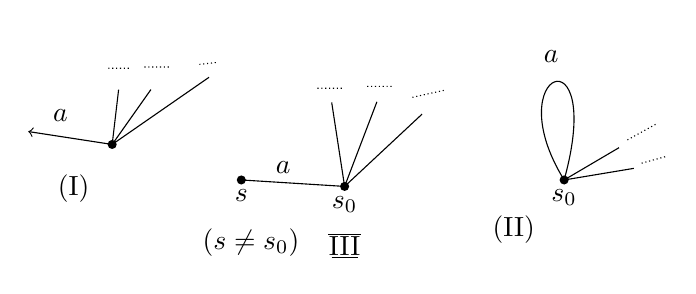
\begin{tikzpicture}[scale=.82]
\fill (0,0) circle (2pt);
\draw[->] (0,0)--(-1.3,.2);\node[above] at (-.8,.2) {$a$};
\draw (0,0)--(.1,.85) (0,0)--(.6,.85) (0,0)--(1.5,1.04);
\draw[densely dotted] (-.06,1.18)--(.26,1.18) (.5,1.2)--(.9,1.2) (1.35,1.24)--(1.62,1.27);
\node[below left] at (-.2,-.32) {$(\mathrm{I})$};
\fill (2,-.55) circle (2pt);\node[below] at (2,-.55) {$s$};
\fill (3.6,-.65) circle (2pt);\node[below] at (3.6,-.65) {$s_0$};
\draw (2,-.55)--(3.6,-.65);\node[above] at (2.65,-.6) {$a$};
\draw (3.6,-.65)--(3.4,.65) (3.6,-.65)--(4.1,.66) (3.6,-.65)--(4.8,.47);
\draw[densely dotted] (3.18,.87)--(3.59,.87) (3.95,.9)--(4.35,.9) (4.65,.73)--(5.15,.84);
\node[below] at (2.15,-1.15) {$(s\ne s_0)$};\node at (3.6,-1.57) {$\mathrm{III}$};\draw (3.35,-1.4)--(3.85,-1.4) (3.4,-1.75)--(3.8,-1.75);
\fill (7,-.55) circle (2pt);\node[below] at (7,-.55) {$s_0$};
\draw (7,-.55)..controls(5.95,1.15)and(7.65,1.8)..(7,-.55);
\node[above] at (6.8,1.12) {$a$};
\draw (7,-.55)--(7.85,-.05) (7,-.55)--(8.08,-.37);
\draw[densely dotted] (7.98,.07)--(8.45,.33) (8.2,-.29)--(8.6,-.18);
\node[below left] at (6.7,-.95) {$(\mathrm{II})$};
\end{tikzpicture}}
\[
T_a=\bigwedge_{\widetilde{a}\in\unsure{A}}T_{\widetilde{a}}\quad
\begin{cases}
T_i&\begin{gathered}\text{dans cas (I) où }i\in J=\widehat{\vec{A}}_{s_0}\text{ est l'élément}\\\text{qui correspond à l'unique }\vec a\text{ sur }a\end{gathered}\\[1.3em]
\displaystyle\bigwedge_{\substack{i\in J\\\text{au dessus}\\\text{de }a}}T_i&\text{dans cas (II)}\\[1.3em]
T_i\wedge_{\{\pm1\}}(\widehat{\vec{A}}_s-\{\vec a\})&\begin{gathered}\text{dans le cas (III),}\\\text{où }\vec a\text{ désigne}\\\text{l'arc d'origine }s\ne s_0\text{ porté par }a\end{gathered}
\end{cases}
\]

On trouve donc
\[
SP_X=\prod_{a\in\widehat{A}}T_a
\]
et avec l'explicitation des $T_a$ par les formules précédentes, on voit que chaque $T_i$ ($i\in J$) intervient dans le produit une fois et une seule, mais sous forme tordue si $i\in J=\widehat{\vec{A}}_{s_0}$ correspond à \unsure{une|un} \unsure{arc|arête} qui est lié et pas une boucle.

Soit donc $\widehat{A}_1\subset\widehat{A}$ l'ens des arêtes de $G$ qui \deleted{\unsure{partent}} n'ont pas \deleted{\unsure{d'autre}} $s_0$ comme extrémité, \deleted{\unsure{liées de par les bords}} \deleted{\unsure{ou que de la contraction}\ \illegible{5}}
\mspage{118}
